% Trailing path operations: -- (axis cs:…) -- cycle with fill opacity,
% a \closedcycle under negative data, and nodes on the plot path by pos.
% Behaviour W1, W4, W5, W6.
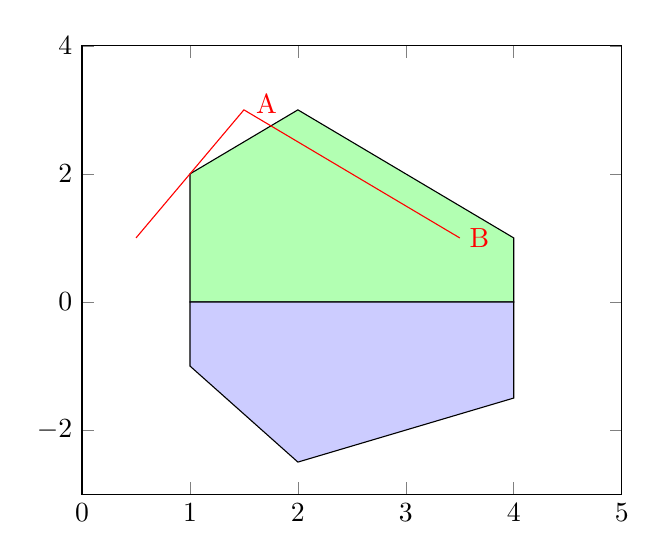
\begin{tikzpicture}
\begin{axis}[xmin=0, xmax=5, ymin=-3, ymax=4]
  \addplot[fill=green, fill opacity=0.3, draw=black] coordinates {(1,2) (2,3) (4,1)} -- (axis cs:4,0) -- (axis cs:1,0) -- cycle;
  \addplot[fill=blue!20] coordinates {(1,-1) (2,-2.5) (4,-1.5)} \closedcycle;
  \addplot[red] coordinates {(0.5,1) (1.5,3) (3.5,1)} node[pos=0.5, above] {A} node[pos=1, right] {B};
\end{axis}
\end{tikzpicture}
